\documentclass[a4paper,12pt]{article}
%\usepackage[latin1]{inputenc}
\usepackage[spanish]{babel}
\usepackage[dvips]{epsfig}
\usepackage{amsmath}
\usepackage{color}
\usepackage{graphicx}
\setlength{\textheight}{235mm}
\setlength{\textwidth}{168mm}
\setlength{\oddsidemargin}{0pt}
\pagestyle{empty}

\begin{document}
\mbox{}\vspace*{-45mm}


{\centering
{\small\sc %Escuela Técnica Superior de Ingenieros de Caminos, Canales y Puertos (Madrid)}\\*[4mm]
Máster Universitario en Ingeniería de Estructuras, Cimentaciones y Materiales}\\*[4mm]
{\Large\bf Método de los Elementos Finitos 24-25}\\*[4mm]
PRÁCTICA 5: Tecnología de elementos. \\*[4mm]}

Se considera una cubierta en forma de bóveda cilíndrica tendiendo un arco de $80^{\circ}$ (figura \ref{fig:esquema}). El material es elástico con módulo de Young $E=432\,\text{MPa}$ y coeficiente de Poisson $\nu=0$.
Las dimensiones son $R=25$ m, $L=50$ m, con espesor $t=0.25$ m.
\begin{figure}[!ht]
\centering
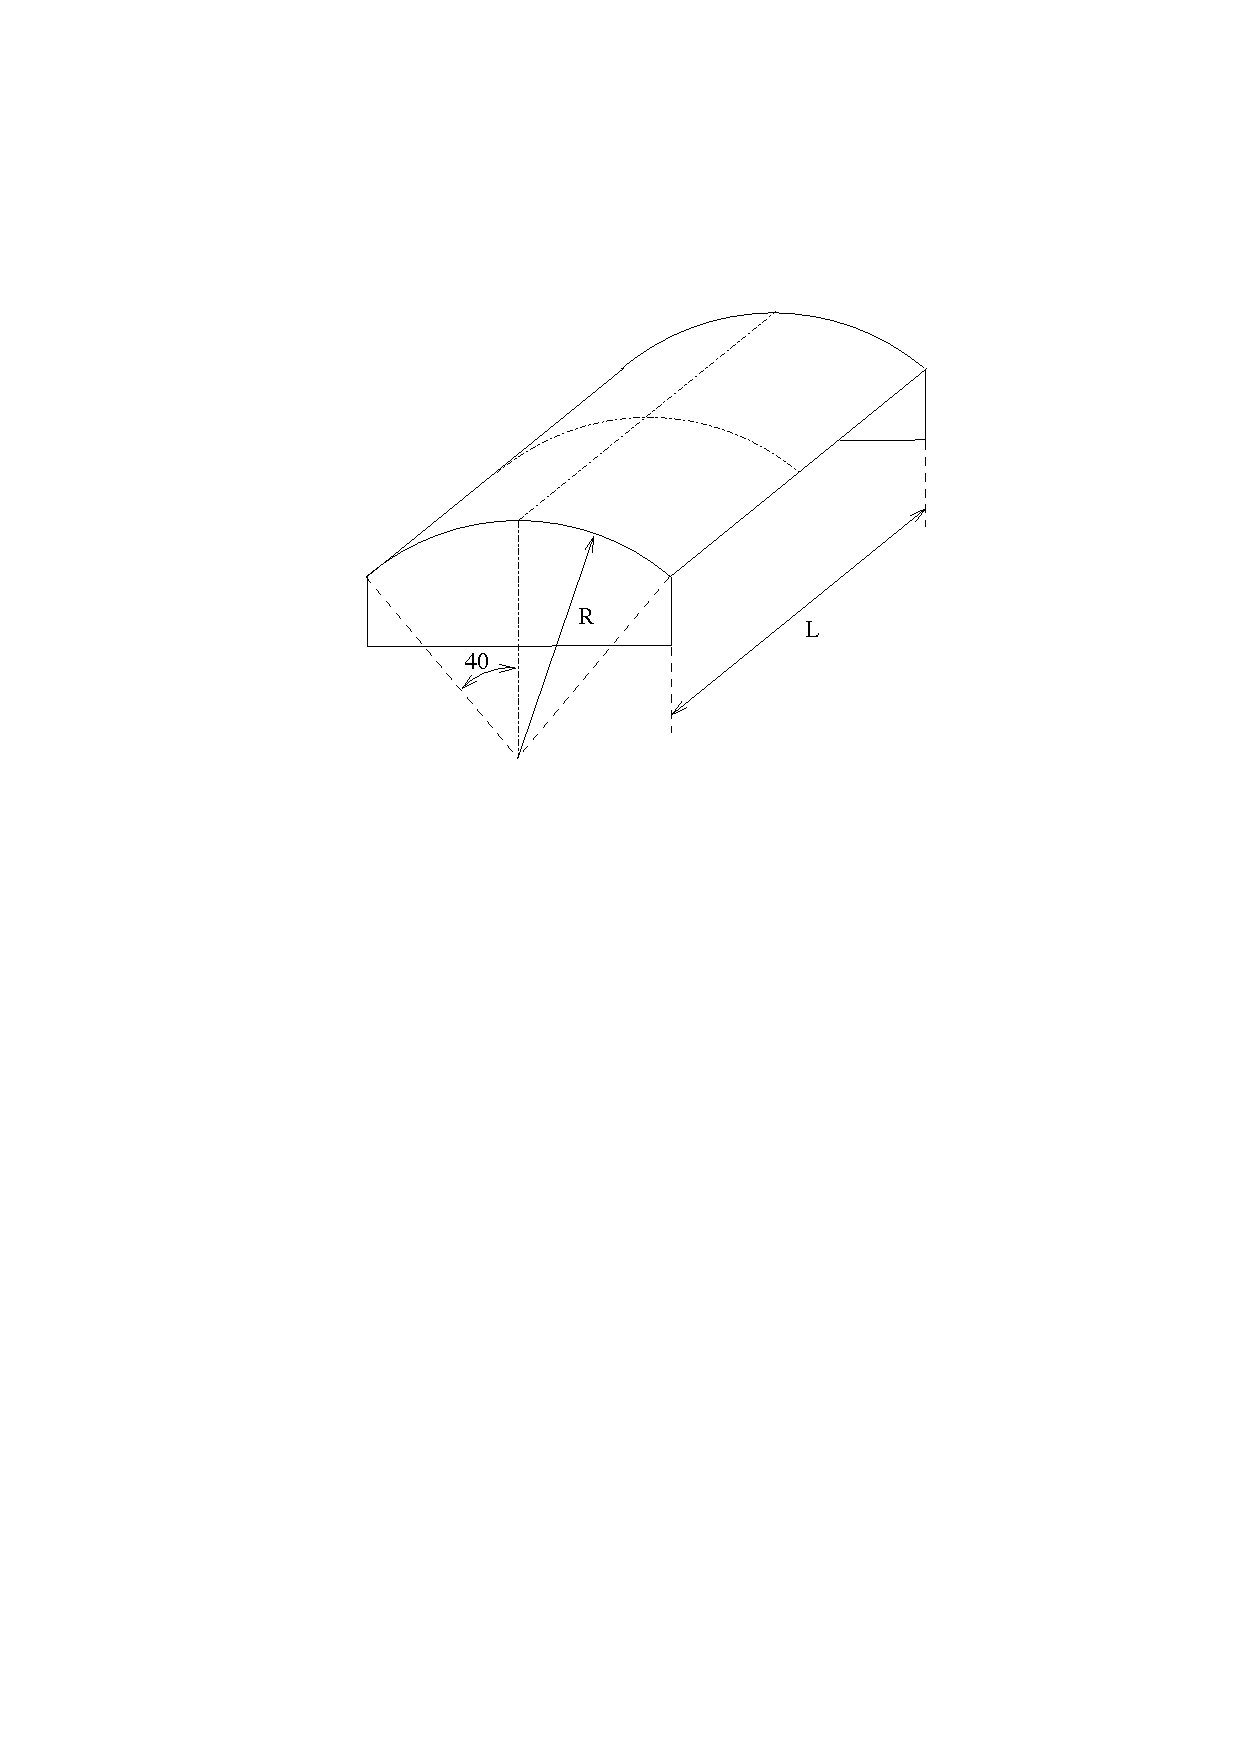
\includegraphics[width=0.5\textwidth]{boveda_scordelis-lo}
\caption{Definición esquemática de la bóveda cilíndrica. }
\label{fig:esquema}
\end{figure}

Los dos extremos curvos están simplemente apoyados sobre diafragmas rígidos, de forma que los desplazamientos en dirección vertical y transversal están impedidos, mientras que el desplazamiento longitudinal es libre. 
Los bordes laterales rectos están libres, sin apoyar.
El conjunto está sometido a su propio peso, siendo el peso específico del material $\gamma=360\,\text{N/m}^{3}$.

\vspace{5mm}

Se pide resolver con elementos sólidos, empleando una discretización de $16\times 16$ elementos y un elemento tan solo en el espesor. Se obtendrá la solución con elementos sólidos hexaédricos de 8 nodos con integración completa (C3D8), con integración reducida (C3D8R), con modos incompatibles (C3D8I) y con formulación mixta (C3D8H).
\vspace{5mm}

El objetivo es obtener como resultado del cálculo los desplazamientos en el borde libre y en el borde superior de la bóveda, así como en la sección central. Asimismo los esfuerzos de momentos flectores en dicha sección central, y las reacciones en los diafragmas.

\vspace{20mm}

\hspace{20mm}\hrulefill$\star$\hrulefill\hspace{20mm}

{\small
\textsc{Nota:} Se trata de un ejemplo clásico de prueba para elementos lámina propuesto por A. C. Scordelis y K. S. Lo, \emph{Computer analysis of cylindrical shells}; J. Amer. Concr. Inst 61, pp. 539-561 (1969).
El resultado de referencia que se puede considerar \emph{``exacto''}, para el desplazamiento vertical en el medio del borde libre, es $0.3024$ m.
}


%\noindent
\end{document}
